%Präambel
\documentclass[paper=a4,fontsize=11pt,headsepline,footsepline,parskip=half]{scrartcl}
\usepackage[utf8]{inputenc}
\usepackage[T1]{fontenc}
\usepackage{amsmath,amsfonts,amssymb}
\usepackage{ngerman,graphicx,textcomp,mathpazo,booktabs}
\usepackage[decimalsymbol=comma,per=frac]{siunitx}
\usepackage[textfont=sl,labelfont=bf]{caption}

%Seite einrichten
\areaset[2cm]		% Zusätzlicher Rand für die Bindung
        {17cm}{24cm}	% Textbreite und -Höhe

%Zeilenabstand
\linespread{1.2} %Standardwert

%Kopf- und Fußzeile
\usepackage{scrlayer-scrpage}
\setlength{\headheight}{23pt}
\lohead{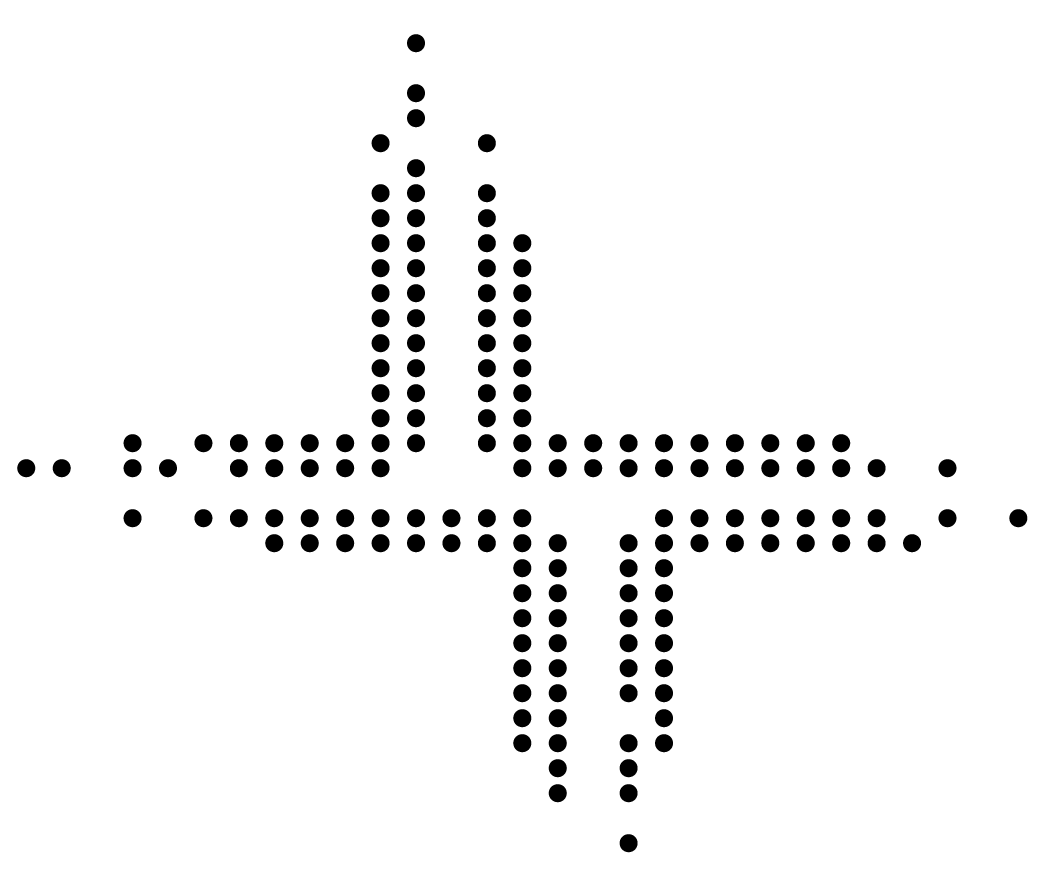
\includegraphics[width=0.7cm]{../logofbi} Hochschule Darmstadt}
\rohead{David Falk, Christian Lichtsinn}
\pagestyle{scrheadings}

\usepackage{subcaption}

%Programmierzeilen
\usepackage{listings}
%Optionen für listings
\lstset{
frame=single, %Rahmen
numbers=left %Zeilennummer
}

%sollte als letztes Paket geladen werden
\usepackage[hidelinks]{hyperref}

\begin{document}

%Titelblatt
\begin{titlepage}

\begin{minipage}[c]{5cm}
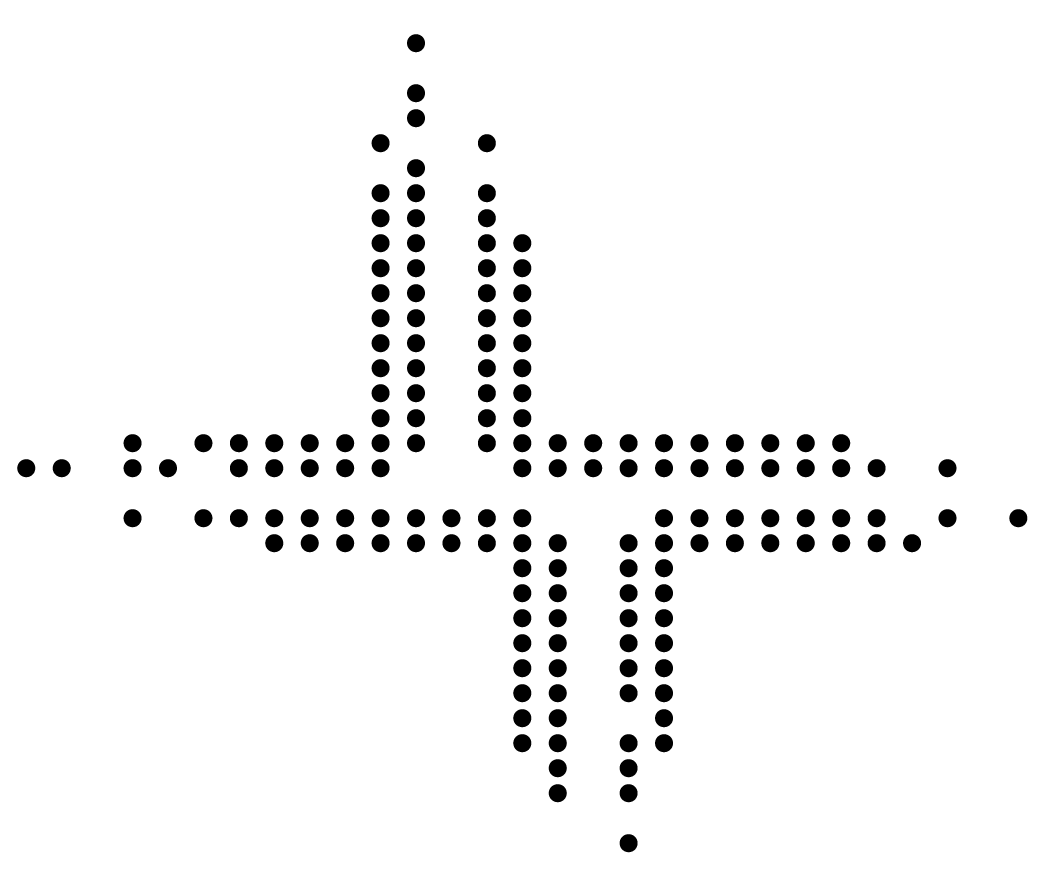
\includegraphics[width=5cm]{../logofbi}
\end{minipage}
\hfill
\begin{minipage}[c]{10cm}
\begin{flushright}
\Large Einführung in die Technik\\und Anwendung von\\
\LARGE \textbf{RFID}
\end{flushright}
\end{minipage}

\vspace*{1cm}

\begin{minipage}[c]{9cm}
\begin{flushleft}
\large David Falk (736532)\\Christian Lichtsinn (736787)\\Praktikum 5 \& 6: 14.12.15 \& 18.01.16: \textbf{Mo-56x}
\end{flushleft}
\end{minipage}
\hfill
\begin{minipage}[c]{7cm}
\begin{flushright}
\large Betreuer:\\Prof. Ralf S. Mayer\\F. Dotzauer
\end{flushright}
\end{minipage}

\vspace*{1cm}

%Workaround nötig wegen parskip Option.
\begingroup
  \setlength{\parskip}{0pt}% keinen Absatzabstand einfügen
  \setlength{\parindent}{0pt}% nicht einziehen
  \setlength{\parfillskip}{0pt plus 1fil}% Absatz darf komplett gefüllt sein
  \par\rule{\linewidth}{1.5pt}\par
\endgroup

\vspace*{\stretch{1}} %stretch zählt all stretch zusammen (hier 1+2=3) und verteilt den vspace entsprechend, hier 1/3

\centering
\Huge{\textbf{\textsl{\huge Dokumentation zur RFID-HF-Applikation\\ \Huge Check das Gepäck!}}}

\vspace*{\stretch{2}} %und hier 2/3 vspace vom Rest der Seite.

\end{titlepage}

\tableofcontents

%KAPITEL 1
\section{Einleitung}

Das Leben als Bodenpersonal eines Flughafens ist kein einfaches. Hier die Piloten, die wesentlich mehr verdienen,
da die Reisenden, die sich demnächst am Strand vergnügen. Und dann das Bodenpersonal, das schnell und ohne große
Komplikation die Reisenden einchecken soll und trotzdem an die Sicherheit denken muss.

Wir schreiben das Jahr 20XX. Inzwischen sind alle möglichen Gegenstände mit RFID-(HF)-Tags versehen. Wäre es doch
toll, wenn das Bodenpersonal ein Programm hätte, mit dem sich schnell und zuverlässig das Handgepäck scannen ließe.

Oh welch ein Glück gibt es \textbf{CheckDasGepäck!} Einfach das Programm starten, kurz scannen und fertig.
Vollautomatisch ohne Knöpfchen drücken. Jetzt muss man nur noch schauen, bei der Arbeit nicht einzuschlafen, weil
man (fast) nichts mehr zu tun hat.

\section{Vorbereitung}

Da das Programm in Java geschrieben ist, funktioniert es grundsätzlich auf jedem Betriebssystem, auf dem Java 8 läuft. Getestet wurde
das Programm in Windows 7.

Außerdem funktioniert das Programm nur in Verbindung mit einem \textbf{scemtec}-Lesegerät, das RFID-HF-Tags auslesen kann. Bevor
CheckDasGepäck! also gestartet wird, sollte man die entsprechende Antenne an den ersten Antennenanschluss des scemtec anschließen,
das Gerät via seriellen Port mit dem PC verbinden und vor allem nicht die Stromversorgung des Geräts vergessen.

Bevor das Programm ausgeführt wird, sollte man vorher noch eine auf manchen Laborrechnern installierte Software Unidemo.exe starten, um
zu schauen, ob der scemtec-Reader auch funktioniert. Unidemo stellt den scemtec dann auch auf die Baudrate 115200, die von CheckDasGepäck!
benötigt wird.

Um das Programm jetzt starten zu können, benötigt man die jar-Datei \textbf{CheckDasGepaeck.jar} und im gleichen Ordner den Ordner \textbf{lib}, 
in dem sich die Bibliothek jssc.jar befindet. JSSC steht für Java-Simple-Serial-Connector, eine Bibliothek, die das programmieren mit seriellen
Schnittstellen vereinfacht. Zudem benötigt man noch eine Datei \textbf{tagid.txt}, die im gleichen Ordner wie CheckDasGepaeck.jar sein muss.

In tagid.txt sind die IDs der Tags festgehalten, sowie welches Objekt sie darstellen sollen und ob dieses Objekt auf ein Flugzeug darf (good)
oder nicht (bad). Die Werte sind mit Leerzeichen getrennt und jede neue Zeile stellt ein neues Tag dar. Beispiel:

\begin{lstlisting}
 383EC34C000104E0 Laptop good
 6C3DC34C000104E0 BigMac bad
\end{lstlisting}

Mit dieser Textdatei weiß das Programm, welcher Tag welchem Objekt zugeordnet wurde und ob das Objekt mit dem
Handgepäck ins Flugzeug darf.

\section{Anwendung}

Ist jetzt alles vorbereitet, dann kann man das eigentliche Programm starten. Entweder mit Doppelklick oder aus der Konsole aus mit:

\begin{lstlisting}
 java -jar CheckDasGepaeck.jar
\end{lstlisting}

Sobald gestartet, muss man gar nichts mehr machen. Das Programm läuft ohne Knopfdruck und erkennt Tags im
Lesefeld automatisch. In Abbildung \ref{fig:app} sieht man, wie das Programm aussieht, wenn es gestartet
wurde und noch keine Tags im Lesefeld sind (\ref{fig:start}), wenn Tags erkannt wurden, die ohne Probleme
mit ins Flugzeug gebracht werden können (\ref{fig:green}) und wie es aussieht, wenn ein Tag erkannt wurde,
das nicht mit ins Flugzeug darf (\ref{fig:red}).

\begin{figure}[th]
  \centering
  \begin{subfigure}[t]{.3\linewidth}
    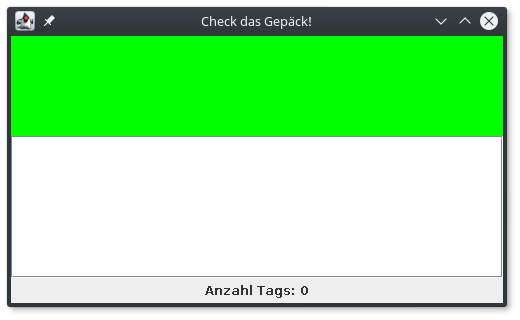
\includegraphics[width=.95\linewidth]{screenshot0}
    \caption{Start ohne Tags.}
    \label{fig:start}
  \end{subfigure}%
  \hfill
  \begin{subfigure}[t]{.3\linewidth}
    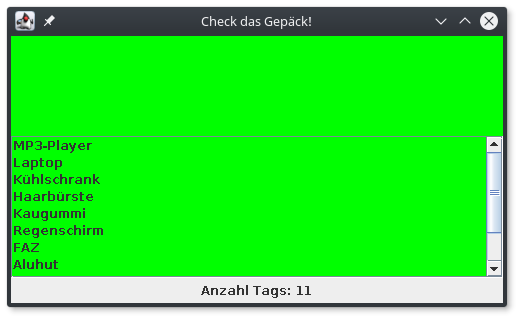
\includegraphics[width=.95\linewidth]{screenshot1}
    \caption{Tags ohne Beanstandung.}
    \label{fig:green}
  \end{subfigure}
  \hfill
  \begin{subfigure}[t]{.3\linewidth}
    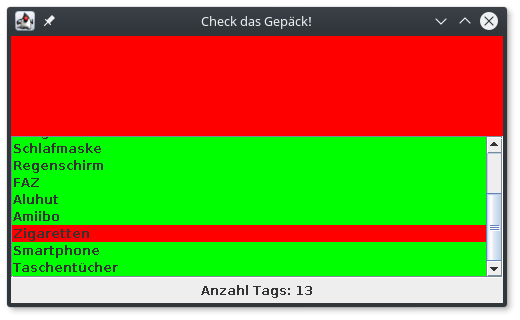
\includegraphics[width=.95\linewidth]{screenshot2}
    \caption{Tags mit Problemen.}
    \label{fig:red}
  \end{subfigure}%
  \caption{CheckDasGepäck! in Aktion.}
  \label{fig:app}
\end{figure}

\end{document}
